\documentclass[preview,border=5pt]{standalone}
\usepackage{teaching}
\begin{document}

\centering

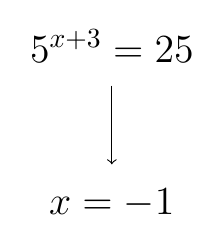
\begin{tikzpicture}[yscale=2,xscale=1,scale=0.5,inner sep=0.3mm, label distance=1.5mm]

\node(t) at (0,1) {\Large $5^{x+3} = 25$};
\draw[->] (0,0.5) -- (0,-0.5);
\node(t) at (0,-1) {\Large $x = -1$};

\end{tikzpicture}

\end{document}